\documentclass[conference]{IEEEtran}

\IEEEoverridecommandlockouts
% The preceding line is only needed to identify funding in the first footnote. If that is unneeded, please comment it out.
\usepackage{cite}
\usepackage{amsmath,amssymb,amsfonts}
\usepackage{algorithmic}
\usepackage{graphicx}
\usepackage{textcomp}
\usepackage{xcolor}
\usepackage{listings}
\graphicspath{{./images/}}
\def\BibTeX{{\rm B\kern-.05em{\sc i\kern-.025em b}\kern-.08em
    T\kern-.1667em\lower.7ex\hbox{E}\kern-.125emX}}
\begin{document}

\title{A Fully Decentralized Infrastructure for Subscription-based IoT Data Trading}
% Chinese title: 針對物聯網資料交易的去中心化基礎建設

\author{\IEEEauthorblockN{1\textsuperscript{st} Ching-Hua (Vivian) Lin}
\IEEEauthorblockA{\textit{dept. of CSIE} \\
\textit{National Cheng Kung University}\\
Tainan City, Taiwan (R.O.C.) \\
jkrvivian@gmail.com}
\and
\IEEEauthorblockN{2\textsuperscript{nd} Ching-Chun (Jim) Huang}
\IEEEauthorblockA{\textit{dept. of CSIE} \\
\textit{National Cheng Kung University}\\
Tainan City, Taiwan (R.O.C.) \\
jserv@ccns.ncku.edu.tw}
\and
\IEEEauthorblockN{3\textsuperscript{rd} Chia-Heng Tu}
\IEEEauthorblockA{\textit{dept. of CSIE} \\
\textit{National Cheng Kung University}\\
Tainan City, Taiwan (R.O.C.) \\
chiaheng@gmail.com}
}

\maketitle


\begin{abstract} 
%cite IoT data subscription economy
The Internet of Things (IoT) makes our lives simple and easier by automating mundane processes with devices around us. Within IoT scenarios, machine-to-machine (M2M) is an inevitable technology that allows machines to own their digital assets and start participating in an economy, which devices can share and trade their resources. The real-time data exchangements among devices are periodically that only data in a specific time period is interested. Thus, publish/subscribe (pub/sub) communication model of streaming data with efficiency and flexibility corresponds such use case. Additionally, the economic layer built on top of subscription-based pricing models as Software-as-a-Service (SaaS) enables monetizing the subscription relationship, which the payment of data streams is calculated with data usage instead of a particular price for a fixed data set. This pricing model allows data providers to have a better vision of managing budgets and data consumers to have the flexibility to subscribe and unsubscribe. However, unlike static data sets, the streaming data increases the importance and difficulties of dynamic data ownership and identity verification. Using certificate authorities (CAs) in such diverse nature for identity verification exposes vulnerabilities of central services, which eventually threaten the trust foundation of the entire system. Therefore, a trustless data trading infrastructure is required where the entities can trade, validate data ownership and data integrity without trusting any service or participants. Besides, consider handling the jobs and trading processes at the same time is too heavy for low-level IoT devices, an automated subscription procedures is also required. In this paper, we leverage usages of distributed ledger techonologies (DLTs) to construct a decentralized and trusted data trading platform on top of the IoT brokered infrastructure. This approach can efficiently enhance the degree of transparency and scalability. The storage via an end-to-end encrypted message streams allows transmitting, accessing and validating data streams over distributed ledgers without authorities, and the trading process is automated through smart contracts. Finally, the prototype is implemented and evaluated.
\end{abstract}

\begin{IEEEkeywords}
Data Marketeplace, decentralization, Distributed Ledger Technology
\end{IEEEkeywords}

\section{Introduction}
In IoT, the development of M2M technology\cite{M2M}, cyber physical system (CPS)\cite{CPS}, and Industry 4.0 grow rapidly. As the physical and digital data are deeply intertwined, the interactions among digital twins act as data exchanges\cite{digitaltwin} which brings potential value to IoT applications, such as health care\cite{healthCare}, factories, and vehicles\cite{AutonomousDriving}, and brings up new business models where data is considered as tradeable digital assets. With the diverse data streams generated by different entities and carried across organizations among expanding amount of interconnected devices, it is a challenge for data holders to share and track their data assets. Therefore, data trading platform is viewed as a solution to build a secure, reliable and scalable data sharing mechanism where data providers and data consumers meet.

%publish/subscribe 的機制符合 IoT 應用情境,因為只在意部份資料
In contrast to the architectures in \cite{DIaas, MARSA} that target to handle static data sets, we aim for processing the high volume, high velocity and high variety of real-time "Big Data" streams\cite{BigData}. As streaming data is composed of records at every moment, users or devices are interested in data of a specific time period instead of the whole timeline. For example, the Internet of Vehicles (IoV) allows vehicles to connect with traffic signs and bicycles, share information, and at the same time be able to understand the real-time environmental conditions and find the best route through the communication. While vehicles and traffic lights continuously generate information, a device only needs to process the data streams of surroundings but all appliances in the IoV. Therefore, the publish/subscribe (pub/sub) communication model that provides the flexibility of following and unfollowing the data streams for users is more appropriate in the IoT scenarios.

% SaaS
The economic incentive model in our proposed IoT data trading platform works as subscription service that valuates the payments by data usage. The subscription-based models (e.g. SaaS and platform-as-a-service (PaaS)) are embedded in our lives, such as newspaper, video/audio streaming and softwares, which can bring enormous operating incomes and offer advantages that allows service providers have the flexibility in resource planning as well as a better prediction of revenue streams. And for service consumers, they can subscribe and unsubscirbe the services at will at anytime. The subscription-based model can easily adapts the underlying pub/sub communication model and benefit both data providers and consumers which promotes a good circulation of the platform. In \cite{SaaS}, the author pointed out that the strength of the relationships between consumers and providers of subscription-based services depends on the service quality (i.e., the data quality in data trading platform), and trust is key to successful subscription-based services.

%trustless & automated
%trust: 對系統、對身份、對資料
In data trading platforms, there are three major aspects that need trust: identity, data ownership and trading. Proving the identity as well as the ownership of data is a challenging issue among various roles in a large scale platform. In current systems, trusted third-party authority like CA is widely adopted to certify each member. However, building trust upon CA is dangerous and fragile. The compromise of routers or CA can break the trust of entire system, and the data portability of using third-party services is still under suspicion. Meanwhile, these concerns are taking into data storage as well, keeping data assets in a centralized data storage or cloud service meet the constraints of data portability, which may violate General Data Protection Regulation (GDPR)\cite{GDPR}. Besides CA and storage, the subscrition history of data consumer may reveal his/hers interests and the exposure of personal information during trading process against GDPR as well. The final trust is trading procedures, apart from setting up the agreement between providers and consumers, both of them need to confirm that the agreement will be executed even if one party fails to comply.

Among the challenges of data trading platform\cite{BigDataMarket} and the requirements mentioned above, we conclude the following four essential ones:
\begin{itemize}
	\item \textbf{Scalability}. 
1) The performance of the platform should scale with the massive amount of participants. 2) The keys and entry points of data products managed by participants should be as small as possible. 
	\item \textbf{Integrity}. 1) Prevent unauthorized modifications. 2) Ensure the accuracy and validity of contents.	
	\item \textbf{Confidentiality}. 
1) Only the authorized participants can access data streams. 2) Participants that have access can always retrieve data even if they're dropped from the network.	
	\item \textbf{Privacy}. Avoid revealing sensitive information of all participants, such as IP address and data consumers' habits which may leak within the subscription history.
	\item \textbf{Economics Incentive}. The economic incentives can encourage the data providers to participate in the system and pay more attention to the quality control. 
\end{itemize}

Taking all the requirements and the features of streaming data into consideration, the data trading platform for IoT towards a decentralized and trustless design. In this paper, we investigate the use of decentralized publish/subscribe (pub/sub) model and DLTs to construct the authority-less and trusted infrastructure. See Fig.~\ref{fig:system_design}. The pub/sub model features the scalability and resource-efficiency, and DLTs resolve the trust of the service, since data and contracts (i.e., smart contracts) written on DLTs are transparent, immutable, and enforced automatically. The trading processes are automated with smart contracts, which allows devices focus on their jobs while gaining the rewards. Lastly, an end-to-end encrypted transmission protocol built on top of DLT is used as data storage, which not only ensures the data integrity, but also enables access control and provides a scalable key and data management.

\subsection{Contributions}
The contributions in the paper are summarized as follow:
\begin{itemize}
	\item Standing on our proposed decentralized data trading infrastructure, we review several decentralized data trading architectures as well as the existing distributed storage, and clarify the necessity of using MAM.  
    \item We make an in-depth analysis of each layer of MAM, in addition to the performance evaluation and optimization of the current implementation. We also compare the perfomance of exchanging different cryptosystems.
	\item We analyze the security concerns when offloading MAM operations to brokers, and propose a solution to resolve them.
\end{itemize}


\subsection{Paper Organization}
The rest of this paper is organized as follows. In Section~\ref{section:relatedWork}, some related work of data exchange mechanisms for IoT, decentralized data trading infrastructures and distributed data storage are analyzed. In Section ARCHI, the design thinking of proposed data trading architecture. In Section ARCHI, the trading models are well explained. The analysis and improvement of MAM are given in Section MAM-EXP. In Section OFFLOAD, the security issues and methods of offloading MAM operations to brokers will be discussed carefully. Finally, we conclude the paper in Section CONCLUSION.

\begin{figure}[!t]
    \centering
    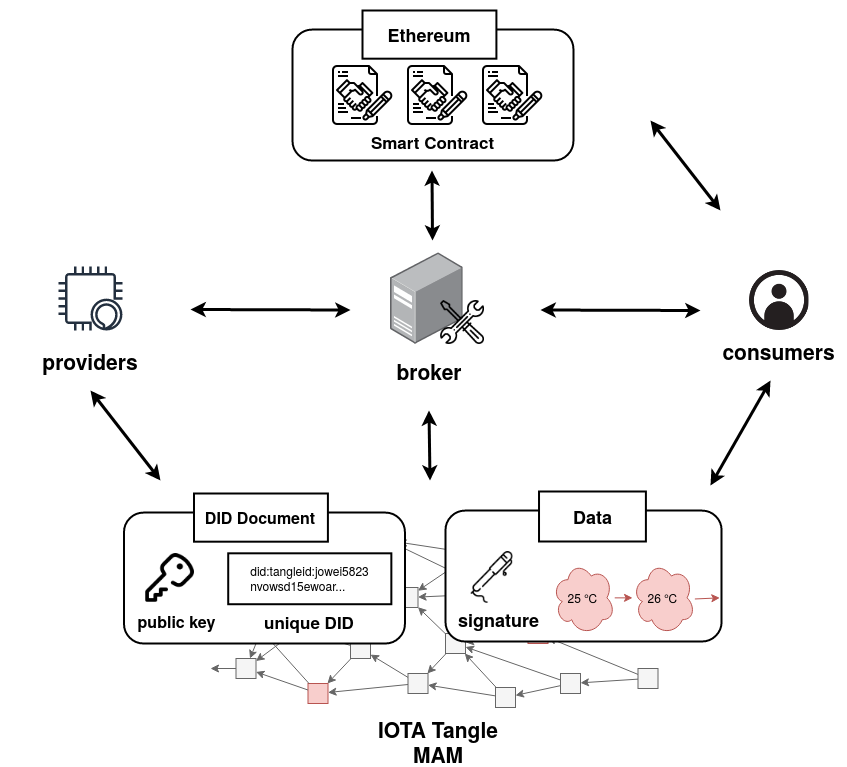
\includegraphics[width=3.in]{system_design}
    \caption{The system design of a decentralized data trading infrastructure which consists of data providers, consumers and brokers.}
    \label{fig:system_design}
\end{figure}

%TODO: cite IOTAIdustryMarketplace
\section{Related Work}
\label{section:relatedWork}
% pub/sub
\subsection{Data exchange mechanism for IoT}
The publish/subscribe service model consists of publishers, subscribers and brokers, which has been proven\cite{pubSubAnalysis, pubSubAnalysis2} to be an efficient and flexible solution for a large number of diverse entities like IoT applications. A lot of work in publish/subscribe system focused on the scalability and the different security issues such as, encrypted data communication, privacy preserving data subscription and access control of digital asset. A few work targets on the storage which is a vital consideration for IoT and mobile computing and the incentive for data economics.

M. B. Abdullahi and G. Wang\cite{centralPubSub} presented a secure publish/subscribe data storage service in Wireless sensor networks (WSNs) which ensures several security issues. Each user has an identity for authentication, whereas subscribers' interests are encoded before matching to protect users' interests. Additionally, the proposed encryption scheme can prevent adversary to access published data if the sensor node is compromised. However, the access control and encryption keys of data is enforced by the network controllers (NCs) and Cirtificate Authorities (CAs), which may be a potential security risk of the system. Also the storage is not well illustrated in the work. G. S. Ramachandran et al.\cite{trinity} pointed out the security risk of centralized brokers, and applied DLTs to build a distributed pub/sub system which promotes the transparency of interactions of participants and the status of data. With the help of Ethereum smart contract, usesrs can perform data validation easily, and brokers can keep track of data status. But data is plaintext on blockchain, which the privacy problem of sensitive data need to be considered carefully. The economics incentives that can encourage the publishers to participate the system and pay more attention on the quality control are not included. 

In \cite{userCentricData}, the publisher runs a node in blockchain that preserves all the history data of the ledger, therefore, they can publish and manage data without any third-parties. The subscribers request publisher directly and ask them to save a cache space for interested data. The main contribution of the system is to ensure data owners have full controls of produced data, but the data owners need to have well devices and environment to perform such functionalities and preserve data. Also, the rights for accessing digital assets is more compatible in the IoT scenarios instead of copying raw data. Secure Pub-Sub model\cite{SPS}, a brokerless of publish/subscribe model, is proposed to eliminate the security risk of middlewares in the model and to provide a reputation-based fairness payment strategy on blockcahin. The privacy and data security are considered thoroughly with the encryption scheme, while the reputation of publishers, payment and data sharing are deployed on smart contracts that allows all operations are transparent. The reputation system and the punishment rules against malicous acts of subscribers and publishers. Yet, without brokers, providers and subscribers may need to reveal more sensitive information like IP address in order to match the both sides. Another broker-less model in \cite{PrivacyPreservPubSub} protects the subscribers' privacy by encrypting users' interests with the light-weight PKEwET\cite{PKEwET}, which allows publishers to match the subscribers' interests in cipher text. 

\subsection{Trusted IoT Trading Infrastructure}
Multiple infrastructures for trusted IoT data trading have been proposed. Paolo Missier et. al\cite{MindMyValue} presented an IoT brokered infrastructure based marketplace which enables trading with Ethereum smart contracts. The brokers are only responsible for data transmission in order to adapt flexible agreement between participants. Unlike the standard pub/sub model that matches publishers and subscribers that participants are unaware of each other. However, the data cubes (i.e., a tuple of information, such as provider, subscriber and time period) are stored in a centralized Cassandra NoSQL database, referring as TrackerDB, is guarateed to be tamperproof but the risk of single point failure still exists. 

\cite{TrustedMarketplaceWearable} focuses on trading the sensitive data among wearables. Several security issues are well discussed and solved with DLTs in the paper, the system consists multiple components that has its different responsibilities, such as data anonymizer eliminates keen information for privacy protection, access controller handles the key management and contract manager manages Ethereum smart contracts. While the trading processes are splited into multiple servers, and the request/response communication model is applied, the scalability problem of the marketplace remains.

In the following researches, IOTA MAM is regarded as a secure data storage which provides access control, tamperproof and authentication functionalities. IOTA is a DAG-based DLT that allows attaching zero value trasactions (i.e., messages) with no transaction fee, and MAM is a protocol that links the messages which forms a channel and endpoint. \cite{luDecentralizedDM} builds the data exchange system with MAM and IPFS\cite{IPFS}, a content-based addressing distributed storage system. Considering the limited transaction processing capability of IOTA, the authors suggest to adopt IPFS to handle the encrypted large data sets, then add the encrypted IPFS link to MAM channel for further exchangement. This research focuses on secure data exchanging architecture design and security analysis, but the trading strategies are not studied yet.

The industrial data marketplace\cite{IOTAIdustryMarketplace} proposed by IOTA Foundation is built on top of IOTA, which targets IoT data streams trading. Data streams are stored via MAM and data payment is paid in IOTA. Nevertheless, the platform design is centralized, where new devices require manual approval to be visible in the marketplace. In \cite{IOTASensorNode}, sensor nodes (SNs) in distributed sensor node system upload data to IOTA network via MAM protocol, and the Back-End server helps SNs to accelerate transaction attachments. The Back-End server also manages keys of data streams, record a tuple of SN, SN metadata, keys and available data stream entry points on MAM, and evaluates data price according to it's quality. Furthermore, as the Back-End server keeps all information of data products, it operates an user friendly interface of the marketplace and tackles all trading procedures. The heavy loading of Back-End server encounters the system scalability problem, single point failure as well as malicious attacks which may damage the profits of all players. 

A similar approach to the previous one, the IOTA-based decentralized data marketplace in \cite{DDMSmartCities} puts data streams via MAM protocol as well. The data marketplace does not exist any intermediate server but data providers only, data providers generate and send data streams to MAM channel, and add a specific tag in transactions as an index that the marketplace application can retreive and show the product information on a map where data consumers can select from. Payments are in IOTA token with the transaction contains another type of tag, which both providers and consumers can double-check. Once the participants grows rapidly, this searching specific transactions by tags approach may fail due to the massive amount of transactions returned. Moreover, it is difficult to filter out the interested information and prevent adversaries spamming useless transactions.  

\cite{SocialGood} proposed a smart transportation system that incorporate two DLTs, IOTA and Ethereum and a distributed storage IPFS. Though IOTA provides better scalability, it does not provide distributed computation as Ethereum smart contract. Thus, in this approach, IOTA and Ethereum are adopted to build a secure and smart system application, which is the principle we followed in our approach. Meanwhile, IPFS and MAM are viewed as the data storage in the system, where IPFS stores data that are not convenient to store on public chain and referenced to its hash into MAM transactions. Three types of MAM channels are used interactively to minimize the channel ID and key that data producers need to manage. However, the access control is examined by Authentication Service, the only client/server communication architecture, where the security issues and bottleneck of system emerges from. Also, the details of trading are not illustrated in this paper.
  
\subsection{Distributed Storage System}
Decentralized storage systems allow users to store files in a distributed network that is maintained by individual nodes around the world instead of a central service provider. Nevertheless, DLTs are often used as the backbone of these systems as data storage and also an incentive layer to encourage people get involved in the network. Filecoin \cite{FileCoin} in Inter-Planetary File system (IPFS) is an incentive layer to incent nodes to provide storage. IPFS is a content-based addressing storage model in a peer-to-peer network, which users can obtain the data with the unique hash value through the network. However, no cryptographic system is applied for user-uploaded files. Sia\cite{Sia} splits the uploaded file into multiple data segments encrypted with the owner's private key, then cipher text is sent to the Sia nodes that rent the storage in Siacoin through smart contracts. Files are duplicated in multiple nodes to prevent data loss.

\section{System Design Thinking}
\subsection{Data subscription-based trading platform players}
There are three major roles, data providers, data consumers and brokers which are similar to the pub/sub messaging model. But unlike the standard pub/sub model where brokers link the publishers and subscribers who are not aware of each others, in our proposed architecture, the brokers are only responsible for message delivery and essential verification processes. As shown in Fig.~\ref{fig:pub_sub_model}.

\begin{figure}[!t]
    \centering
    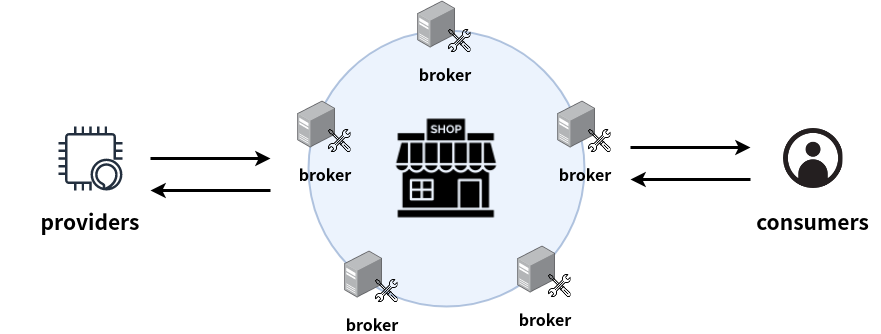
\includegraphics[width=3.in]{pub_sub_model}
    \caption{The players in data subsciption-based trading platform consists of data providers, data consumers and brokers.}
    \label{fig:pub_sub_model}
\end{figure}

\begin{itemize}
\item \textbf{Data Provider: }
Data providers are the ones that generate streaming data and set the data price based on the different types of data. With the subscription fee that earned via trading, data providers are incentivized to maintain and improve the quality of data.
\item \textbf{Data Consumer: }
Data consumers are entities that are willing to buy data streams. As it is laborious to widely deploy devices to collect data from scratch, and without a marketplace, it is also difficult to find providers of the data sets, purchases is the fastet and efficient way to get the desired data sets. 
\item \textbf{Broker: }
Brokers are responsible for building an agreement between data providers and consumers. Also brokers can represent data providers to perform computing tasks as brokers are expected to have higher resource. 
\end{itemize}

We adopt the brokered infrastructure for three reasons. Firstly, it inherits the benefits from the standard pub/sub model which is more efficient than the request/response model specifically in a large scale system. Furthermore, if either side is offline, the proceeding tasks have to stop and start over. With brokers, the unfinished work can be cached or accomplished. Second, a fully decentralized architecture has difficulties to brings data providers and consumers together, both of them need to reveal more sensitive information, such as IP address, in order to build the communication tunnel. The existence of brokers resolved the privacy issue, as brokers are the bridges that link data providers and consumers, participants can trade with minimum info like its identifier and public key. Third, as brokers running on machines in a stable network and electricity environment, besides matching procedures, participants on resource-constrained devices can offload the computation tasks to brokers. In our proposed protocol, devices can delegate the uploading and trading processes to brokers after signing the data, and brokers can perform verifiable checks without knowing the contents.           

\subsection{Choice of Data Storage}
Data storage is the trust basis of data trading platforms where the data assets are reserved. Streaming data unlike a fixed set of data which can be verified by the hash of whole pack of data, it consists of continually granular records of each time slots. Therefore, the verification such as, data integrity and source identity are narrow down to a data point as well. In our proposed architecture, we adopt Masked Authenticated Messaging (MAM)\cite{MAM} as data storage to resolve the challenges of managing and verifying data streams. MAM is the second layer data communication protocol built on top of IOTA\cite{IOTAwhitepaper} network, the Tangle, a feeless cryptocurrency designed for IoT, which introduces properties like publishing, classifying and tracking authenticated message streams. 

In our work, MAM build the trust of the platform while meeting the requirements of data trading which can be concluded below:

\begin{itemize}
    \item \textbf{Scalability}: For both data providers and consumers, MAM keeps the number of managed keys and data entry points as small as possible
    \item \textbf{Integrity}: 
	\begin{itemize}    	
    	\item Messages published to the Tangle are tamperproof that against malicious modification. 
    	\item Messages are signed with the keys pre-generated under Merkle signature scheme\cite{MSS} (MSS) that both keys and messages can be verified by participants.
    \end{itemize}
    \item \textbf{Confidentiality}:
    \begin{itemize}    	
    	\item The encrypted data are uploaded that only participants that have keys can decrypt. 
    	\item The authorized users can retrieve data streams, since data is written on the Tangle which can be queried as long as the IOTA network is alive.
    	\item MAM provides forward-secrecy. The entry points of future data can be derived, but it's impossible to trace back those in the past. This feature prevents adversaries from retrieving published history even if the key is revealed.
    \end{itemize}
\end{itemize}

MAM publishes authenticated streaming data to channel and endpoint as zero-value transactions to the Tangle and provides the ability to publish and fetch encrypted messages over the network along with data integrity and access control. The payload of a MAM message can be encrypted with an \textbf{encryption key} that restricts only authorized players can access contents, the ciphertext is then signed with \textbf{signature key} generated with MSS and attached to the Tangle. This approach allows users to validate the signatures without knowing the actual contents but ensuring the messages do come from the exact source. See Fig.~\ref{fig:channel_and_key} for illustration. Furthermore, the rights of data access are traded instead of a copy of data in the trading platform, which eliminates the need for data consumers to have additional storage. 

\begin{figure*}[!t]
    \centering
    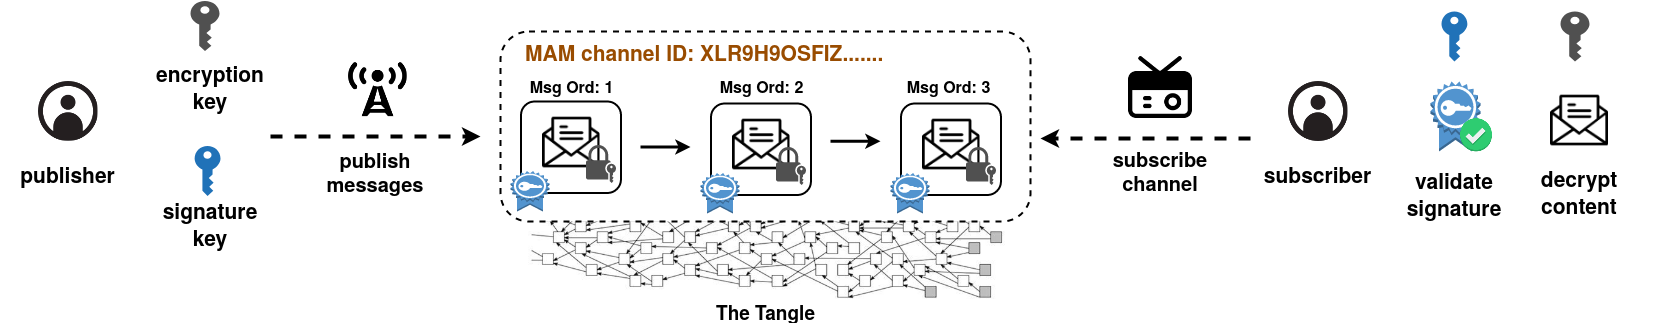
\includegraphics[width=\linewidth]{channel_and_key}
    \caption{Within MAM channel, the message publisher has 2 types of key, the encryption keys for content encryption and signature keys for digital signatures. Subscribers can validate the message with signature keys and decrypt messages with encryption keys.}
    \label{fig:channel_and_key}
\end{figure*}

% alternative solution => IPFS(data) + MAM(index)
\subsection{Digital Identity}
The digital identity represents an entity and holds the digital assets within the digital world, it is important to prove and show the identity to others during interactions. In our architecture, a self-soverign identity system TangleID\cite{TangleID} is used to manage the identity information that allow entities to prove its identity without any third-party authority. TangleID is built on top of MAM where change log of the Decentralized Identifiers (DIDs)\cite{DID} defined by W3C is traceable. The identity information such as public key, unique identifiers of services and metadatas consist a DID document. One can easily prove himself by sharing the identifier on MAM without any authority. 

Through TangleID, every entity gets a public/private key pair, the location of DID document and the seed that generates the DID document MAM public channel. The public/private key pair can be used to exchange sensitive data and establish the trust communication, where messages that are encrypted with a public key can only be decrypted with private key owner. During data subscription process, the encryption keys of data products are encrypted with data consumers' public key on DID document which ensures only the subscribed consumers are accessible.

\subsection{Enable Automated Trading Process}
Ethereum is a cryptocurrency building on top of a public blockchain-based distributed ledger. It provides the smart contract, which is a protocol for formulating agreement on a blockchain that running on decentralized virtual machines. A smart contract can interact with other contracts, make decisions, store data and transfer cryptocurrency. All the participants in Ethereum can verify and execute the contracts, and once the contract is triggered, it is uninterruptible and will be executed automatically without any third-parties. 

With the functionalities of Ethereum smart contracts, a flexible and verifiable trading mechanism can be acheived. In our system, \textbf{Product Contract} is made for the product launching and trading. The information of data products such as address of the data provider, subscription fee, brokerage fee, threshold of consent votes of refunding, MAM channel/endpoint ID (the data entry point), time period and the broker-verified encryption key are listed on Product Contract. See Listing. \ref{lst:constructor}. Furthermore, the participants can exchange encryption keys without any authorities via smart contracts. Though this design may cost extra transaction fees than exchanging key off-chain, it is considered a more secure strategy to protect the privacy of participants.

The transparency of smart contracts bring advantages for data providers and consumers. One of the advantage is that the trading states and progress are visible and verifiable which profits providers and consumers respectively. For data providers, with every details opened, the consumer list functions like a reputation evaluation, the better the quality the more the consumers he/her has. The consumer list and the states of products, which includes \textit{Launched, KeyCertified, Finished} and \textit{Refunded} are key reputation referenced for data consumers to decide whether to subscribe. 

\lstdefinestyle{solidity}{
	captionpos=b,
	tabsize=4,
	basicstyle=\scriptsize
}
\lstset{style=solidity}
\begin{lstlisting}[caption={Product Contract data fields}, label={lst:constructor}, frame=single]
contract Product {
    address public broker;
    address public provider;
    bool isBrokerWithdraw;
    bool isProviderWithdraw;
    address[] consumers;
    
    struct Purchase {
        bool affirmativeVote;
        bool isConsumerWithdraw;
        bool isKeyAdded;
        string encryptKey;
    }
    mapping(address => Purchase) public consumer2Purchase;
    
    uint public price;
    uint public totalAmount;
    uint public brokerage;
    uint public threshold;
    string public channelRoot;
    string public endPoint;
    uint public totalNumber;
    uint public uploadedNumber;
    uint public affirmativeVotes;
    string blindedKey;
    string signedBlindedKey;
    
    enum State {Launched, KeyCertified, Finished, Refunded}
    State public state;
}
\end{lstlisting}

\subsection{Enable delegation of computation tasks to broker}
To participate data subscription, data providers have to interact with MAM and Ethereum smart contract while doing its original tasks. However, the resources of low-level devices are precious which should be used to focus on its jobs. Therefore, the operations of MAM and smart contracts are better to be delegated to brokers. 

The delegation should also ensure the privacy of data providers, for instance, brokers are asked to attach messages to MAM without knowing the contents as well as record encryption keys to smart contracts. To deal this issue, we use blind signature\cite{blindSig} to allow brokers to certify and update the sensitive contents without knowing it. Blind signature is a form of digital signature where the message is first "blinded" by a random "blinding factor", then passed to a signer to sign. Figure \ref{fig:blind_signature} illustrates the steps of blind signature. The resulting message, along with the blinding factor, can be later verified with the signer's public key. 
% TODO: redraw blind signature diagram
% TODO: broker 進行簽章的必要性

RSA blind signature\cite{cryptoNote} is used in our research. The user chooses a random number $r$ and uses the signer's public key $e$ to generate a blinding factor $r^e$. To prevent the message $m$ from being known by the signer, the user sends blinding message $c$ to the signer instead of $m$.

\begin{equation}
C = r^e m
\end{equation}

The signer signs the blinding message with his private key $d$.

\begin{equation}
S = C^d
\end{equation}

$S$ is the signer's signature of $C$. In RSA system, $ed$ is equal to 1. To remove the blinding factor, the user computes the following calculation.

\begin{equation}
\frac{S}{r}= \frac{C^d}{r} = \frac{(r^e m)^d}{r} = \frac{r^{ed} m^d}{r} = m^d
\end{equation}
 
The user gets $m^d$ which is the signer's signature of the message $m$. At the same time, the signer does not know $m$ and the session key is protected. 

\section{Masked Authenticate Messaging}
Data storage is the trust basis of data trading platforms where the data assets are reserved. Streaming data unlike a fixed set of data which can be verified by the hash of whole pack of data, it consists of continually granular records of each time slots. Therefore, the verification such as, data integrity and source identity are narrow down to a data point as well. In our proposed architecture, we adopt Masked Authenticated Messaging (MAM)\cite{MAM} as data storage to resolve the challenges of managing and verifying data streams. MAM is the second layer data communication protocol built on top of IOTA\cite{IOTAwhitepaper} network, the Tangle, a feeless cryptocurrency designed for IoT, which introduces properties like publishing, classifying and tracking authenticated message streams. Carrying these properties, MAM is also appropriate for building a self-soverign identity system where the identity information such as public key, unique identifiers of services and metadatas are stored. One can easily prove himself by sharing the identifier on MAM without any authority. 

MAM publishes authenticated streaming data as zero-value transactions to the Tangle and provides the ability to publish and fetch encrypted messages over the network along with data integrity and access control. With MAM, the rights of data access are traded instead of a copy of data in the trading platform, which eliminates the need for data consumers to have additional storage. Channel and endpoint represent a stream of messages, which functions as singly-linked lists. The singly-linked list structure implements the concept of forward secrecy, where no one has access to the data back from his/her entry point. Furthermore, each address of a message can be derived from the previous one, which enables data consumers to subscribe to future data by having the endpoint ID. A MAM channel/endpoint ID is the address of a transaction and the first message of a channel/endpoint. The central endpoint in Fig.~\ref{fig:mam_struct} means its endpoint ID is the same as channel ID. 

A user can create multiple channels and endpoints, and the messages can be encrypted with the session key then broadcasted in chronological order to the Tangle by attaching it to an endpoint. This allows only authorized entities are able to decode these messages after retrieving them from the Tangle. 

\begin{figure}[!t]
    \centering
    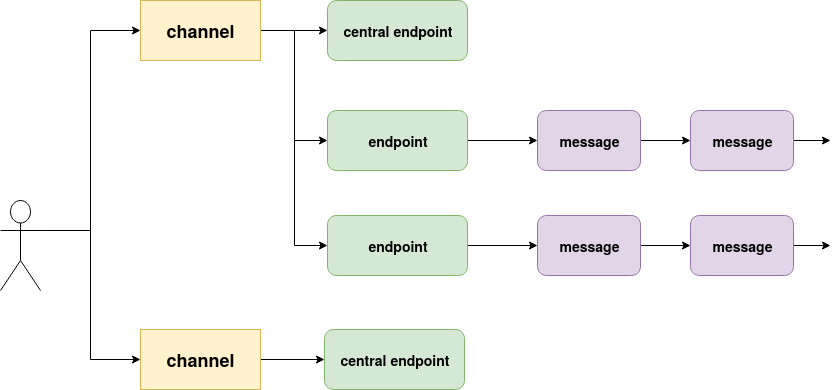
\includegraphics[width=2.5in]{mam_struct}
    \caption{The concept of MAM.}
    \label{fig:mam_struct}
\end{figure}

The authentication in MAM includes two aspects: source and data. Source authentication ensures the message that originates from the claimed owner, and data authentication ensures the integrity of the data from that sender. These are achieved through the MSS which is a digital signature scheme based on Merkle Hash Trees and One-way hash functions. However, the size of Merkle Hash Trees, that is, the size of a channel/endpoint should be determined at the start. Thus, data providers need to first decide how to distribute data products into MAM channels/endpoints before uploading data. Using MAM as a data storage benefits from the scalability of the underlying IOTA network as well as the decentralized and fault-tolerant characteristic of distributed ledgers, which reduce the risks of centralized storage services. 

%scalability
The importance of scalable key and data entry points management increases as the service operating over time. In MAM, with an entry point (i.e., the address of transaction) and the encryption key, one can derive the following addresses of transaction and retrieve data. Table.~\ref{tab:mam_scalability} compares the key and addresses that need to be managed by using MAM and other distributed storage systems. Assuming the length of data stream is 7, and each record is encrypted with the same key. With MAM, only 1 key and 1 entry point is required while other distributed storage need to reserve 7 entry points for each data record.

\begin{table}[htbp]
	\caption{Number of keys and entry points of a data stream that need to managed with length 7.}
	\label{tab:mam_scalability}
	\begin{center}
	\begin{tabular}{|c|c|c|}
	\hline
		\textbf{Items} & \textbf{MAM} & \textbf{Others} \\ 
		\hline
		keys & 1 & 1 \\ 
		\hline
		entry points & 1 & 7 \\ 
		\hline
	\end{tabular}
	\end{center}
\end{table}

%classify
The channel and endpoint structures enable users to be able to easily categorized data streams with respect to different types and usages. For instance, a voice assistant can create a channel every day with multiple endpoints for each gadgets to record daily logs. Another example is sensor devices like AirBox\cite{LASS}, collects environmental data, can split the statitics like PM 2.5 and humidity by time period into separate channels, which is useful for data providers to organize records and to pack into different data products. To do the classification in other distributed storage also encounters the aforementioned scalability problem, data entrypoints of the data steams should be reserved.    

%data trace
Moreover, data tracability is an important security issue that allows users to track the changes of data. Currently, hash is widely used to generate checksums of entire package of files, users can compare the hash value of files in order to check the integrity. Yet the hash values of each new version are unrelated and it's hard to point out the differences between versions. MAM benefits from the singly linked-list data structure which attaches messages chronologically, users can easily track the footprints of data change logs as well as checking the validity of modifications with the signature.

The operations of MAM are frequent, especially for data providers, who either upload data in a short time interval or maintain multiple MAM channels or endpoints at the same time, hence the operation of MAM is one of the potential bottleneck in data marketplace. In this paper, we evaluate the performance of MAM, and improve the effeciency with different strategies. Also, we take offloading the computation tasks to brokers as another possiblie approach for IoT devices, since brokers are considered to have higher computating power.

\section{Decentralized Data Marketplace Case Study}
Trading Models of Decentralized Data Marketplace
\subsubsection{Set Up}
All participants need to register on TangleID\cite{TangleID}, a self-soverign identity system built on top of MAM, enables authentication without any third party via a decentralized identifiers and a public/private key pair for authentication. 

\subsubsection{Launch Data Products}
To launch a data product, data providers need to create a MAM channel/endpoint and a Product Contract. However, considering IoT devices have no ability to handle both uploading data to MAM and interacting Ethereum smart contracts while collecting continuous data with low computing power, these works are offloaded to brokers. 

The details of data product, such as data price, MAM channel/endpoint ID and time period are listed on the Product Contract. As regard to the encryption key of data product, it is certified by a broker with blind signature\cite{blindSig}, a mechanism that allows users to sign contents without knowing it, and written the signed key on the Product Contract. This provides an approach for data consumers to verify the encryption key that avoid data providers frauding data consumers with a wrong one. The workflow is shown in Fig.~\ref{fig:launching_product}. 

Data providers start uploading data once the MAM channel/endpoint are created, each MAM message contains encrypted contexts along with signatures which allows data consumers to check the integrity. In addition, one can perform the signature validation without the encryption key on MAM.
 
\begin{figure}[!t]
    \centering
    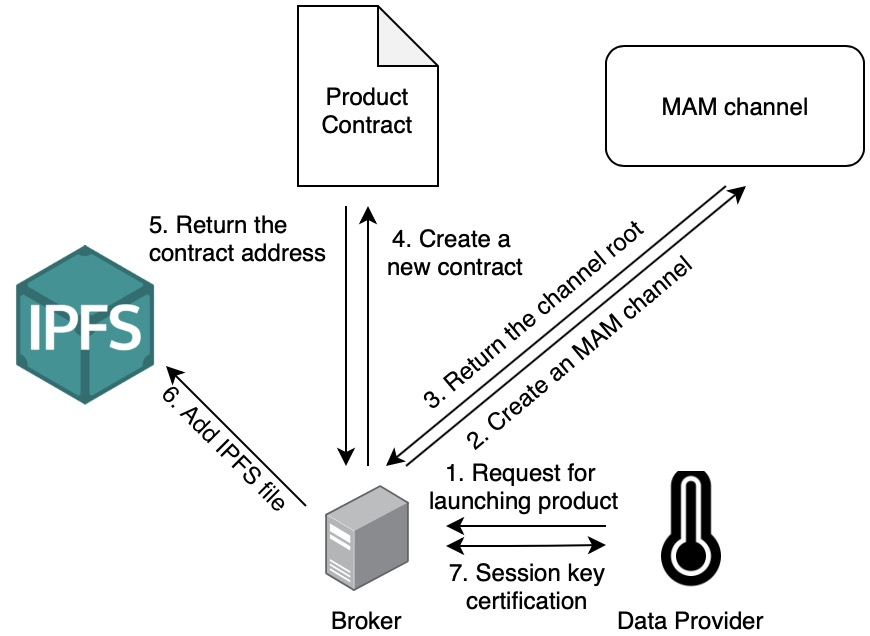
\includegraphics[width=2.5in]{launching_product}
    \caption{The process of launching a product.}
    \label{fig:launching_product}
\end{figure}

\subsubsection{Trading}
Data consumers pay subscription fees to the Product Contract of desired data products, and data providers give the "access" of data products on MAM instead of the files to consumers. The MAM channel/endpoint encryption key is encrypted with the public key of data consumer by data provider and written on the Product Contract, which ensures only data consumers can retreive it from Product Contract. 

Transferring the encryption key on smart contract instead of off-chain not only ensures the consistency of the encryption key but also prevents frauds from malicious participants. Furthermore, with the help of brokers and smart contracts, both data providers and consumers do not need to be online at the same time to proceed the trading process. The key sending process is shown in Fig.~\ref{fig:key_exchange}. 

\begin{figure}[!t]
    \centering
    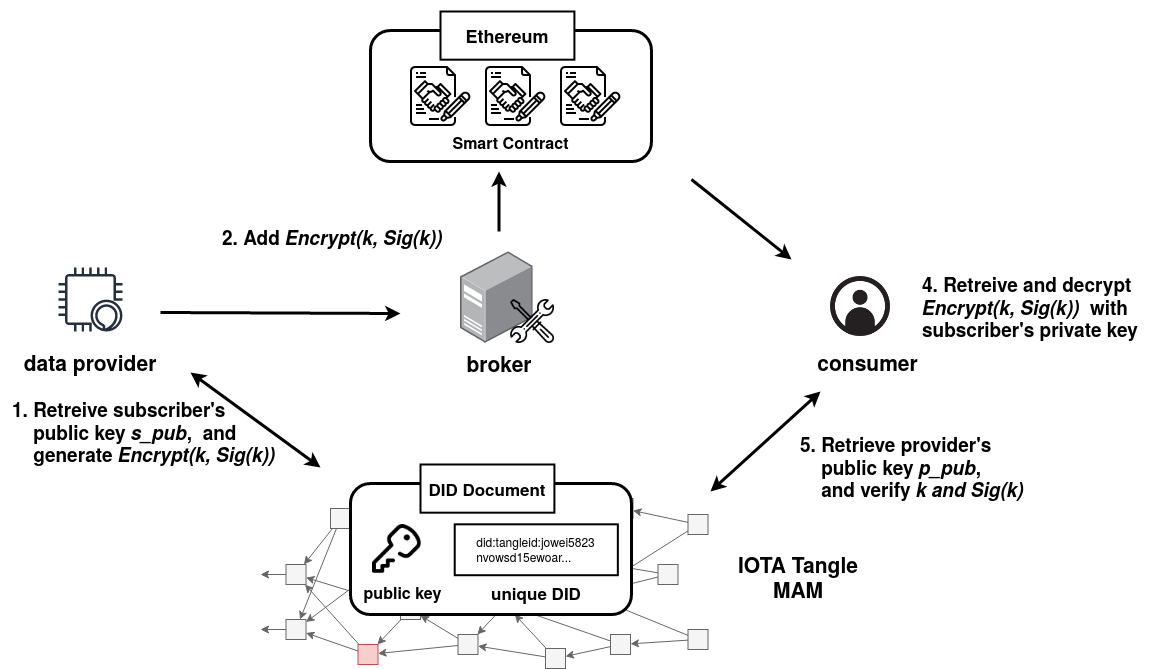
\includegraphics[width=3.5in]{key_exchange}
    \caption{Encryption key exchangement process.}
    \label{fig:key_exchange}
\end{figure}

\subsubsection{Refunding}
Subscribing to future data is a high-risk which data provider may not upload data as the agreement set after recieving the subscription fee. Therefore, in our proposed architecture, data consumers can initiate a refund procedure if the data is not available or defective. The subscription fee is transferred from the Product Contract to data providers when the committed data is available on MAM. When the refund procedure is launched, all consumers start voting based on their opinions on the data product. Once the ratio of consent votes of refunding is higher than a threshold, the subscription fee is proportionally transferred to the data provider, broker and every consumer. 


\section{Evaluations}
It is worth making a claim that all participants in data marketplace do not need to hold an IOTA full node which maintains the transaction history and exchanges information of the Tangle. Each role is only required to run client libraries and communicate with IOTA full nodes to interact with the Tangle. Therefore, in the following evaluations, all devices run with client library only.

\subsection{MAM Performance Evaluation}
MAM is a secure and validatable data storage of the proposed architecture. And publishing data to MAM is the primary key to resolve all the difficulties discussed in previous sections. The interactions between data providers and MAM can be frequent. Data providers can either upload data in a short time interval or maintain multiple MAM channels or endpoints at the same time, hence the operation of MAM is one of the potential bottleneck in data marketplace.

In this section, time measurement is evaluated in two MAM operations: channel/endpoint creation and data attachment to endpoints. To perform the evaluation assessment, a personal computer (PC, 3.2GHz 64-bit 6-core i7-8700 with 16GB DDR4 RAM) and a Raspberry Pi 3 Model B (1.2 GHz 64-bit quad-core ARM Cortex-A53 with 1GB LPDDR2 RAM) have been used to run MAM. 

\subsubsection{Channel / Endpoint Creation}
The length of a channel or endpoint is $2^{height}-1$ where \textit{height} is the height of Merkle Hash Tree in a Merkle signature scheme (MSS), and the "$-1$" is for announcing the ID of next channel or endpoint. A channel with height $n$ can create $2^n-1$ endpoints, and an endpoint with height $m$ can attach $2^m-1$ messages, therefore the capacity of a channel is $2^{nm}-2^n-2^m+1$ messages in total. The greater the \textit{height} of MSS, the longer the channel/endpoint, however the higher the computational power required. In this task, both channel and endpoint creation are tested and the \textit{height} is set from 1 to 7 which is quite enough for data providers to upload data. The results are shown in Table \ref{tab:channel_create} and Table \ref{tab:endpoint_create}. The time duration for each \textit{height} is the average time of running 100 rounds.

\begin{table}[htbp]
	\caption{Time measurement of channel creation}
	\label{tab:channel_create}
	\begin{center}
	\begin{tabular}{|c|c|c|}
	\hline
		\textbf{height of MSS} & \textbf{PC (sec)} & \textbf{Raspberry Pi 3 (sec)} \\ 
		\hline
		1 & 0.26183 & 2.908702 \\ 
		2 & 0.524076 & 5.805524 \\ 
		3 & 1.045942 & 11.555660 \\ 
		4 & 2.092989 & 23.178036 \\ 
		5 & 4.19515 & 46.164079\\ 
		6 & 8.361586 & 92.320173\\ 
		7 & 16.651607 & 185.292243\\
		\hline
	\end{tabular}
	\end{center}
\end{table}

\begin{table}[htbp]
	\caption{Time measurement of endpoint creation}
	\label{tab:endpoint_create}
	\begin{center}
	\begin{tabular}{|c|c|c|}
	\hline
		\textbf{height of MSS} & \textbf{PC (sec)} & \textbf{Raspberry Pi 3 (sec)} \\ 
		\hline
		1 & 0.256425 & 2.887064 \\ 
		2 & 0.505679 & 5.767912 \\ 
		3 & 0.999524 & 11.550455 \\ 
		4 & 1.994017 & 23.260508 \\ 
		5 & 3.965007 & 46.748366 \\ 
		6 & 7.918925 & 93.182975 \\ 
		7 & 16.561419 & 186.064562 \\
		\hline
	\end{tabular}
	\end{center}
\end{table}

The results of Table \ref{tab:channel_create} and Table \ref{tab:endpoint_create} are plotted in Fig.~\ref{fig:mam_create}. Since the creation of channel and endpoint are MSS calculations, the curves of the same hardware are nearly identical. On the other hand, the performance of Raspberry Pi 3 is acceptable when \textit{height} is smaller than 4, but time grows rapidly when \textit{height} is 5 or above. And the performance of PC remains acceptable even \textit{height} gets to 7. The results indicate that MAM channel/endpoint creation is a laborious job for a Raspberry Pi 3 when data providers need a longer channel/endpoint, which is one of the reason that MAM operations should be forwarded to brokers.
  
\begin{figure}[!t]
    \centering
    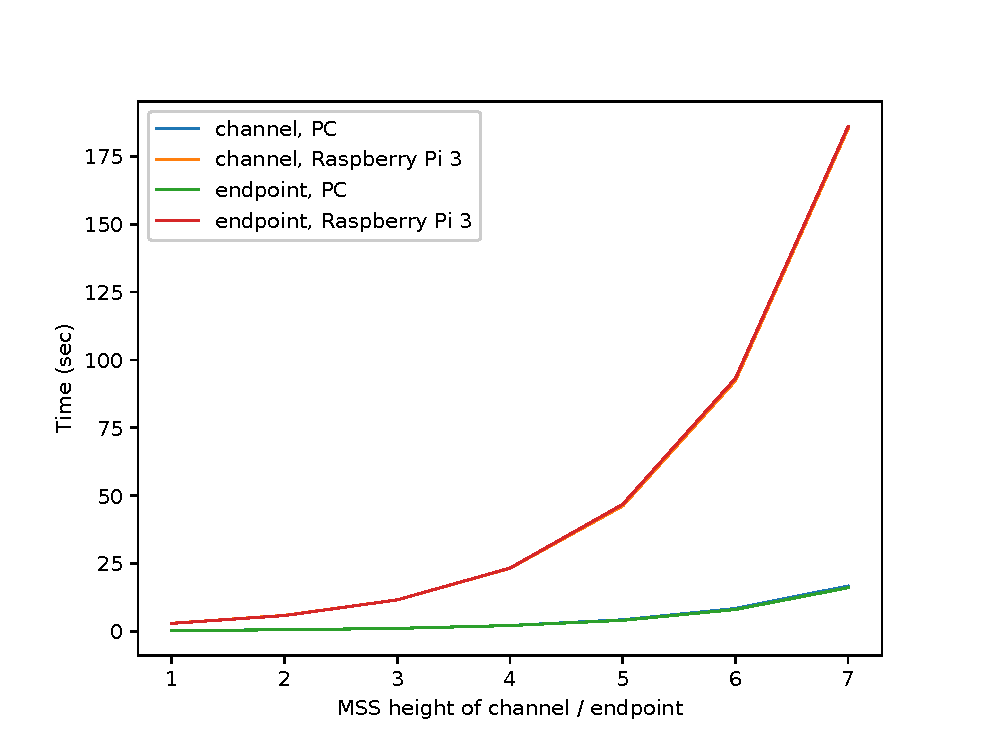
\includegraphics[width=2.5in]{mam_create}
    \caption{Time cost of MAM creation.}
    \label{fig:mam_create}
\end{figure}

\subsubsection{Messages Publishment}
Publishing a message to MAM is attaching a zero-value transaction to the Tangle which requires two processes:
\begin{itemize}
	\item	Tips selection: In the IOTA protocol, a new-coming transaction needs to pick up 2 existed transactions called tips to reference and verify. The tips are provided by IOTA full nodes.
	\item	Proof-of-Work (PoW): An algorithm which prevents Denial of Service and spam attacks on a network. A computationally hard puzzle to solve, but easy to verify. IOTA uses a Hashcash\cite{Hashcash} based puzzle.
\end{itemize}

Tips selection requires a stable network connection to wait the response from IOTA full nodes, and PoW requires enough computation resources to perform. Fig.~\ref{fig:mam_send} shows probability distribution function of publishing a message to MAM endpoint. The time of Raspberry Pi 3 distributed widely, since the randomness of PoW has huge impact while all the tests on PC remain in a possible range.

\begin{figure}[!t]
    \centering
    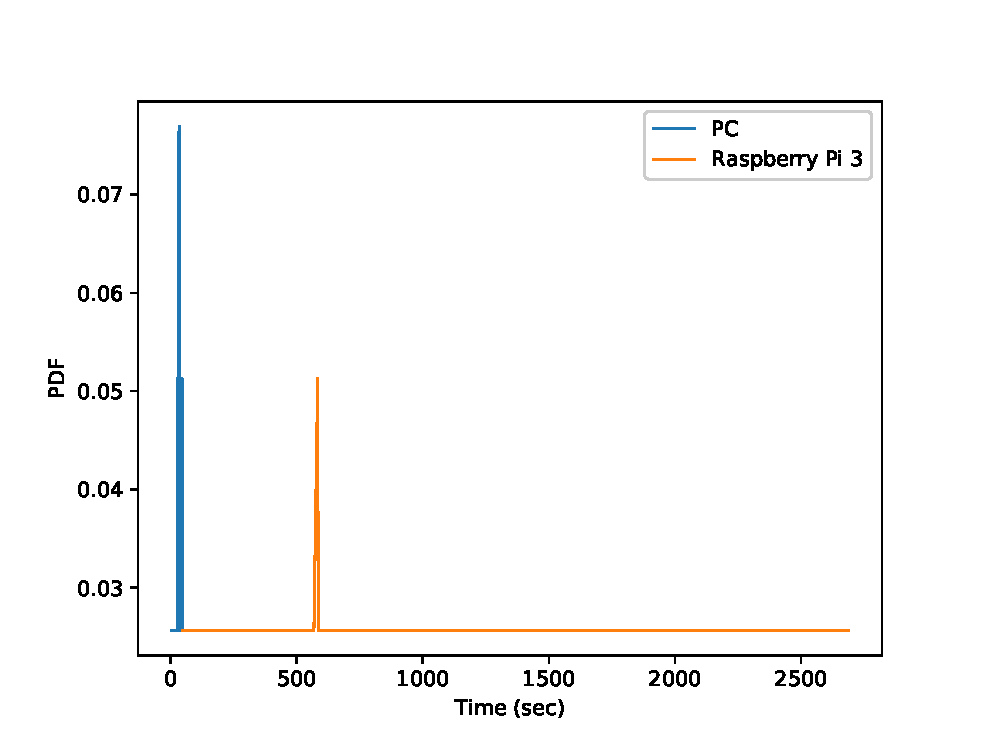
\includegraphics[width=2.5in]{mam_send}
    \caption{Time cost of sending a message through MAM.}
    \label{fig:mam_send}
\end{figure}

The simulation results above indicate that MAM is difficult for low-level sensor devices to run, whereas these kind of devices are the majority hardware in the IoT scenarios. Furthermore, sensors with the low computing power and unstable internet connection are not able to have enough resources to handle data collection, data transmission on MAM and even trading process with subscribers simultaneously. 

Therefore, transferring MAM operations to brokers while ensuring the profit and privacy of providers through blind signatures can effectively solve performance problems and lower the threshold to participate in such framework. Brokers can be PCs or powerful machines that runs Ethereum client and Tangle-accelerator\cite{TA}. Where Ethereum client is used to interact with Ethereum and Tangle-accelerator is a caching proxy server for IOTA, which can serve thousands of IOTA requests at once without accessing remote IOTA full nodes frequently and provide PoW acceleration. Fig.~ \ref{fig:ta_struct} shows the structure of Tangle-accelerator. However, MAM operations still cost a considerable time that improving the performance of MAM is an essential issue that needs to be done for the next step.  

\begin{figure}[!t]
    \centering
    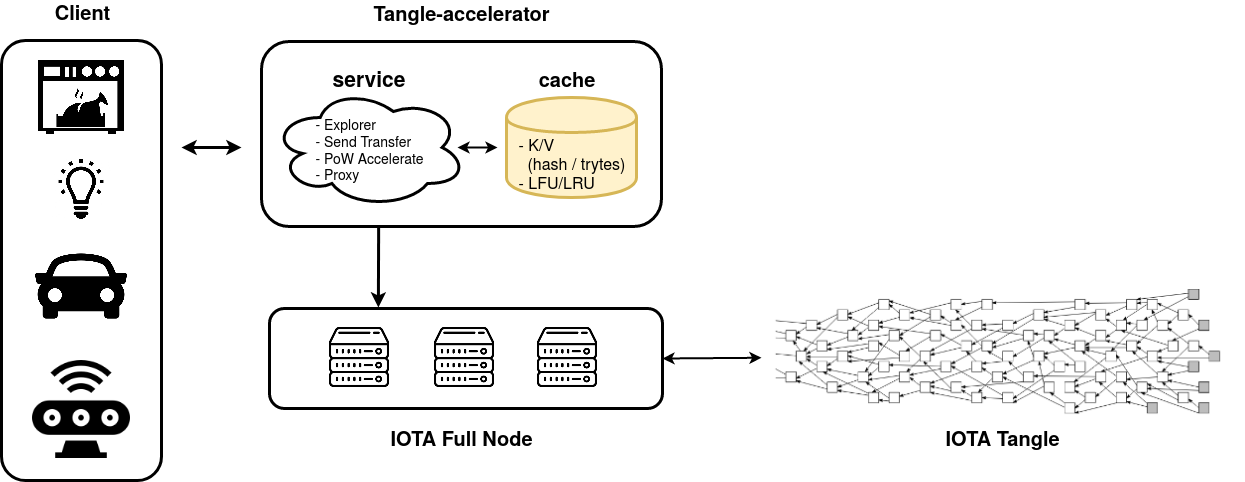
\includegraphics[width=3in]{ta_structure}
    \caption{The structure of Tangle-accelerator.}
    \label{fig:ta_struct}
\end{figure}

\section{Conclusions}
By combining the established standards and openly-developed specifications, this paper proposed an autonomous publish/subscribe model design to serve as a vendor and industry-neutral platform, automating the trading of digital assets and services. It was built with blockchain network, immutable audit trails, and contracts with an integrated decentralized identity system, to ensure the authenticity of all participants and enable secure communication and flexible trading mechanisms.

\bibliographystyle{IEEEtran}
\bibliography{references}

\end{document}
